\documentclass[12pt]{article}
\author{Alex Ho}
\title{FYS4150 - Computational Physics \\ Project 2}
\usepackage{listings}
\usepackage{graphicx}
\usepackage{verbatim}
\usepackage{amsmath}
\usepackage[utf8]{inputenc}
\usepackage[english, norsk]{babel}
\usepackage{xcolor}
\usepackage{hyperref}

\lstset{
language=Python,
basicstyle=\ttfamily,
otherkeywords={self},             
keywordstyle=\ttfamily\color{blue!90!black},
keywords=[2]{True,False},
keywordstyle={[2]\ttfamily\color{blue!90!black}},
emph={MyClass,__init__},          
emphstyle=\ttfamily\color{red!80!black},    
stringstyle=\color{blue!90!black},
showstringspaces=false,
commentstyle=\color{blue!90!black},
breaklines=true,
tabsize=3,
moredelim=**[is][\color{blue}]{@}{@}
}

\begin{document}
\maketitle
\section{Introduction}
In this project, we will have a look at the so called \textit{Eigenvalue problem}. We will use the well known Schrödinger equation from quantum mechanics and apply it to a system consisting of a single electron in a harmonic oscillator potential. To achieve this, we will implement Jacobi's method to solve the Schrödinger equation and then find the eigenvalues, which will physically be the energies of the electrons.

We will also look at the case where we have two interacting electrons in a three dimensional harmonic oscillator, with different frequencies.
\section{Method}
\subsection*{2a) Mathematical intermezzo}
We first want to look at the orthogonality properties of a specific basis. Let us consider the following basis of vectors
\begin{align}
\mathbf{v}_i = \begin{pmatrix}
v_{i1} \\
v_{i2} \\
\vdots \\
v_{in}
\end{pmatrix}
\end{align}
We will also assume that this is an orthogonal basis
\begin{align}
\mathbf{v}_j^T\mathbf{v}_i = \delta_{ij}
\end{align}
We want to look at the orthogonality properties for a orthogonal and unitary vector transformation in the form
\begin{align}
\mathbf{w}_i = \mathbf{U}\mathbf{v}_i
\end{align}
For an orthogonal matrix, we know that $\mathbf{U}^T\mathbf{U} = \mathbf{I}=1$, where $\mathbf{I}$ is the identity matrix, so we have that
\begin{align}
\mathbf{w}_j^T\mathbf{w}_i = (\mathbf{U}\mathbf{v}_i)^T(\mathbf{U}\mathbf{v}_i) = \mathbf{v}_j^T \mathbf{U}^T\mathbf{U}\mathbf{v}_i = \mathbf{v}_i^T\mathbf{v}_i = \delta{ij}
\end{align}
For a unitary matrix, we have that $\mathbf{U^*}\mathbf{U}=\mathbf{I}$ and $\mathbf{U}^{\dagger}\mathbf{U} = \mathbf{I}$, where $\mathbf{U}^{\dagger} = (\mathbf{U}^*)^T$ is the hermitian conjugate. Doing the hermitian conjugate on the transformation vector, we can show that
\begin{align}
\mathbf{w}_j^{\dagger}\mathbf{w}_i = (\mathbf{U}\mathbf{v}_j)^{\dagger}(\mathbf{U}\mathbf{v}_i) = \mathbf{v}_j^{\dagger}\mathbf{U}^{\dagger}\mathbf{U}\mathbf{v}_i = \mathbf{v}_j^{\dagger}\mathbf{v}_i = \delta_{ij}
\end{align}
Here we have assumed that the basis vector is real, so $\mathbf{v}_i^* = \mathbf{v}_i$.
\subsection*{2b) Jacobi's rotation method}
Jacobi's rotation method (or Jacobi's method) is an algorithm that can be used to solve the eigenvalue problem. Consider an $n\times n$ orthogonal transformation matrix
\begin{align}
\mathbf{S} = \begin{pmatrix}
1 & 0 & \cdots & 0 & 0 & \cdots & 0 & 0 \\
0 & 1 & \cdots & 0 & 0 & \cdots & 0 & 0 \\
\cdots & \cdots & \cdots & \cdots &\cdots & \cdots & \cdots & \cdots \\
0 & 0& \cdots & \cos \theta & 0 & \cdots & 0 & \sin \theta \\
0 & 0 & \cdots & 0 & 1 & \cdots & 0 & 0 \\
0 & \cdots & \cdots & \cdots & \cdots \\
0 & 0 & \cdots & 0 & 0 & \cdots & 1 & 0 \\
0 & 0 & \cdots & -\sin\theta & 0 & \cdots & 0 & \cos\theta
\end{pmatrix}
\end{align}
with the property $\mathbf{S}^T = \mathbf{S}^{-1}$. A similarity transformation, on a matrix $\mathbf{A}$
\begin{align}
\mathbf{B} = \mathbf{S}^T \mathbf{A} \mathbf{S}
\end{align}
gives us 
\begin{align}
b_{ii} &= a_{ii} ,\quad i\neq k, i\neq l \\
b_{ik} &= a_{ik} \cos\theta - a_{il}\sin\theta, \quad i\neq k, i\neq j \\
b_{il} &= a_{il}\cos\theta + a_{ik}\sin\theta, \quad i\neq k, i\neq j \\
b_{kk} &= a_{kk}\cos^2\theta - 2a_{kl}\cos\theta\sin\theta + a_{ll}\sin^2\theta \\
b_{ll} &= a_{ll}\cos^2\theta + 2a_{kl}\cos\theta\sin\theta + a_{kk}\sin^2\theta \\
b_{kl} &= (a_{kk}-a_{ll})\cos\theta\sin\theta + a_{kl}(\cos^2\theta - \sin^2\theta)
\end{align}
The angle $\theta$ is arbitrary. The idea here is to choose a $\theta$ that causes all non-diagonal matrix elements to become zero (or within a given tolerance). However, not all non-diagonal matrix elements will become zero after one iteration, so we will have to run this algorithm a sufficient amount of times to get the desired result.

First we have to choose a value $a_{ij}$. This value will be the largest non-diagonal value in the matrix $\mathbf{A}$ and needs to be larger within a tolerance $\epsilon$, that is
\begin{align}
\text{max}(a_{ij}^2) > \epsilon
\end{align}
Since we want the non-diagonal matrix elements to become zero, we require that $b_{kl} = b_{lk} = 0$, which gives
\begin{align}
b_{kl} = (a_{kk} - a_{ll})\cos\theta\sin\theta + a_{kl}(\cos^2\theta - \sin^2\theta) = 0
\end{align}
Defining $\tau = \frac{a_{ll}-a_{kk}}{2a_{kl}}$ and $\tan\theta = t = \frac{\sin\theta}{\cos\theta}$, we can write the above expression as
\begin{align}
-2a_{kl}\tau t + \frac{a_{kl}}{\cos^2\theta}(\cos^2\theta - \sin^2\theta) &= 0 \nonumber \\
\implies -2\tau t + 1 - t^2 &= 0 \nonumber \\
\implies t^2 + 2\tau t - 1 &= 0
\end{align}
Where we have in the first line inserted the expression for $\tau$ and then divided by $\cos^2\theta$. We can now use this second order equation to determine $\tan\theta$.
\begin{align}
\tan\theta = -\tau \pm \sqrt{1+\tau^2}
\end{align} 
Once that is determined, one can easily calculate the new values of $\cos\theta$ and $\sin\theta$ given as
\begin{align}
\cos\theta &= \frac{1}{\sqrt{1 + \tan^2\theta}}\\
\sin\theta &= \cos\theta \tan\theta 
\end{align}
When these are calculated, we can compute the new values of $b$ which results in a new matrix. We then repeat the same procedure, with this new matrix, until
\begin{align}
\text{max}(a_{ij}^2) > \epsilon
\end{align}
is no longer satisfied. The end result is that the matrix $\mathbf{A}$ will only contain values along the diagonal, which will be the eigenvalues (or energies) of the system. Note that the eigenvalues along the diagonal are not ordered from the lowest to highest eigenvalue (or vice versa).

The reason we decided to choose the largest value of the non-diagonal elements is because of this test. It ensures that all the non-diagonal elements will be close to zero, thus giving us the diagonal matrix with the desired eigenvalues.
\section{Implementation}

\section{Results}
In the C++ program, by selecting the number of mesh points to $n=400$, with $\rho_{max} = 10$, the output for the non interacting case is the following:
\begin{lstlisting}
@
Using a 400x400 matrix (n = 400)
with rho_max = 10

Time elapsed for non interactive case: 305.675s
Number of iterations: 260506
Lowest 3 eigenvalues are: 
2.99981
6.99903
10.9976
Possible number of orthogonal vectors: 79800
Number of orthogonal vectors: 79800
Number of non-orthogonal vectors: 0
@
\end{lstlisting}
The eigenvalues, even though they are not within 4 decimal precision, are very close to the exact analytical eigenvalues. We can also see that the number of iterations needed to fully diagonalize the matrix $\mathbf{A}$ (or at least within a tolerance $\epsilon$) was 260506 iterations. The unit test of the orthogonality between the eigenvectors is also shown, where every possibly combination of the scalar product between the eigenvectors are orthogonal (also within a tolerance).

The time it took for the program to run was roughly 5 minutes. This seems like a very long simulation time, so there is probably something that is not quite optimal in the program, thus causing the program to run for a longer time.

Figure 1 shows the the probability distribution of the wave function (or the eigenvectors we calculated) for different frequencies $\omega$.
\begin{figure}[hbtp]
\centering
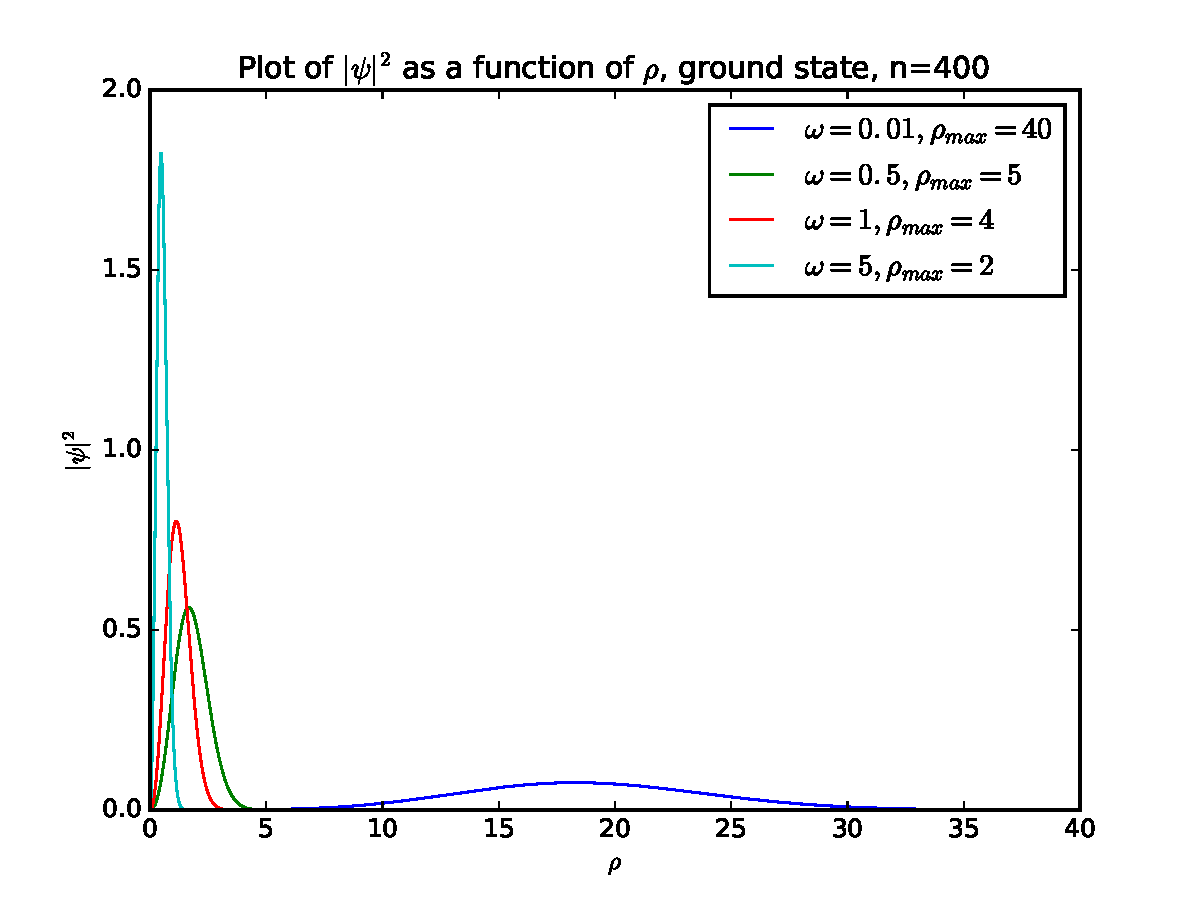
\includegraphics[width=\linewidth]{Plots/Plot_groundstate_n400.pdf}
\caption{Probability distribution of the wave functions of the ground state, for different values of $\omega$. Plotted for $n=400$ meshpoints.}
\end{figure}
These results are not quite surprising. Let us for a moment imagine that two electrons are bound together by a spring. The electrons oscillate back and forth due to the oscillation of the spring. They interact once when they are closest to each other (that is, the distance between them is the minimum).

For lower frequencies, the electrons will interact less frequently which means, by the analogy above, they are further apart from each other a lot more often. Another way to think of this is that the spring can be drawn over a larger distance before it is forced to contract, thus allowing the electrons to go further out. This can be seen from figure 1 (the blue line with $\omega = 0.01$) where the probability of them being close to each other is very small, while them being further apart is slightly larger.

For higher frequencies, the electrons will interact more frequently. Using the same analogy, we can think of the electrons bouncing back and forth very quickly. The spring is very stiff, so it cannot be stretched that far. Because of this, the electrons are forced to be very close to each other, which is exactly what we see in figure 1. In the case of $\omega = 5$ (the cyan line), we can clearly see that the probability of them being very close to each other is very large, while them being further apart is very low (practically zero).
\section{Conclusion}

\section{References}
M. Hjort-Jensen, 2015, \textit{Computational Physics}, accessible at course GitHub repository; \url{https://github.com/CompPhysics/ComputationalPhysics/tree/master/doc/Lectures} (as of 14.09.16), 551 pages.
\end{document}